 %%	SECCION documentclass																									 %%	
%%---------------------------------------------------------------------------%%
\documentclass[a4paper]{report}

%%---------------------------------------------------------------------------%%
%%	SECCION usepackage																											 %%	
%%---------------------------------------------------------------------------%%
\usepackage{amsmath, amsthm}
\usepackage[spanish,activeacute]{babel}
\usepackage{caratula}
\usepackage{a4wide}
\usepackage{hyperref}
\usepackage{fancyhdr}
\usepackage{graphicx} % Para el logo magico!
\usepackage{amssymb}
\usepackage{amsmath}
\usepackage[latin1]{inputenc}
\usepackage[dvipsnames,usenames]{color}
\usepackage{amsfonts}
\usepackage{ulem}
%\usepackage{highlight}
\usepackage{fancybox}
%\usepackage{marvosym}

%%---------------------------------------------------------------------------%%
%%	SECCION opciones																												 %%	
%%---------------------------------------------------------------------------%%
\parskip    = 11 pt
\headheight	= 13.1pt
\pagestyle	{fancy}
\definecolor{orange}{rgb}{1,0.5,0}

\addtolength{\headwidth}{1.0in}

\addtolength{\oddsidemargin}{-0.5in}
\addtolength{\textwidth}{1.0in}
\addtolength{\topmargin}{-0.5in}
\addtolength{\textheight}{0.7in}

%%---------------------------------------------------------------------------%%
%%	SECCION document	 %%	
%%---------------------------------------------------------------------------%%
\begin{document}
\renewcommand{\chaptername}{Parte }

%%---- Caratula -------------------------------------------------------------%%
\materia{Ingenier�a del Software II (2do cuatrimestre de 2009)}
\titulo{Trabajo Pr�ctico I - Preentrega}

\integrante{Castillo, Gonzalo}{164/06}{gonzalocastillo\_086@hotmail.com}
\integrante{Elizalde, Victoria}{452/06}{kivielizalde@gmail.com}
\integrante{Gonzalez, Sergio}{481/06}{gonzalezsergio2003@yahoo.com.ar}
\integrante{Page Saal, Mart�n}{315/06}{martinpage2001@yahoo.com.ar}
\resumen{
En el siguiente documento, se arribar� la fase de elaboraci�n del proyecto relacionado con la implementaci�n de un sistema de mediciones telem�tricas, que unir� puntos estrat�gicos del pa�s con el fin de capturar la informaci�n necesaria y procesarla, para anticiparse a los diferentes fen�menos meteorol�gicos. En dicha fase se identificar�n y detallar�n las funcionalidades principales del sistema y si arquitectura b�sica. Adem�s se definir� un plan detallado para esta segunda iteraci�n del proyecto.}

% TOC, usa estilos locos
\maketitle
\pagestyle{empty}
{
\fancypagestyle{plain}
    {
    \fancyhead{}
    \fancyfoot{}
    \renewcommand{\headrulewidth}{0.0pt}
    } % clear header and footer of plain page because of ToC
\tableofcontents
}

\newpage
% arreglos los estilos para el resto del documento, y
% reseteo los numeros de pagina para que queden bien
\pagenumbering{arabic}
\fancypagestyle{plain} {
    \fancyhead[LO]{Castillo, Elizalde, Gonzalez, Page Saal}
    \fancyhead[C]{}
    \fancyhead[RO]{P\'agina \thepage\ de \pageref{LastPage}}
    \fancyfoot{}
    \renewcommand{\headrulewidth}{0.4pt}
}
\pagestyle{plain}

\newpage
\chapter{An�lisis de entorno y enunciado}

Al leer el enunciado, una de las primeras veces, surg�an nuevas terminolog�as y se mencionaban tecnolog�as no conocidas, que en este proyecto ten�an gran importancia. Por este motivo fue necesario investigar ciertos aspectos, para introducirse en el tema y poder comprender mejor el dominio del problema al que nos est�bamos enfrentando.

Una vez hecho esto, se pudo identificar con mas facilidad los requerimientos primarios del sistema y pudimos observar adem�s del gran tama�o del proyecto, que exist�an ciertos factores de complejidad y disponibilidad en cuanto a los datos y a los modelos que se necesitaban manejar. Por esta raz�n, pensamos que no era una buena idea, tener todo el sistema centralizado y se comenzaron a identificar partes que realicen diferentes tareas de forma tal de distribuir y organizar mejor la funcionalidades. Por esta raz�n se decidi� modularizar la Estaci�n Central y las Terminales Remotas. Dentro de la Estaci�n Central se pudieron identificar varias partes que se desprend�an de la descripci�n del proyecto: Pudimos identificar una parte encargada del procesamiento de los datos que llegaban de las TRs, asi tambi�n del uso de los mismos para realizar las predicciones; Otra de las partes era la destinada al intercambio de informaci�n con clientes externos o usuarios que monitoreaban el sistema, estos servicios tienen en com�n que pueden ser realizados mediante web services, uno de los requerimientos para realizar la comunicaci�n con clientes externos; Y un sistema de almacenamiento, con un backup de la informaci�n, para evitar la perdida de datos. En cuanto a la Terminal Remota, se pudo identificar lo siguiente: Una parte central, encargada de la recepci�n de los datos enviados por los sensores, y de el env�o de estos en el momento oportuno, todo esto con su correspondiente almacenamiento para aquellos datos que fueron enviados, pero no fueron confirmados; Las dem�s partes son componentes f�sicos que se agregan a la TR, pero que es bueno identificarlos para tener una mejor visi�n de la TR, estos son las baterias, los paneles solares, el componente muy usado del mercado, y los sensores.Para tener entonces una idea de las diferentes partes del sistema, se realizo un diagrama contextual mostrando y relacionando las diferentes partes mencionadas. El mismo de alguna forma sirve tambi�n como un primer diagrama de arquitectura, ya que, en el se identifican los diferentes componentes f�sicos y la comunicaci�n entre ellos.

\begin{figure}[!hbt]
\centering
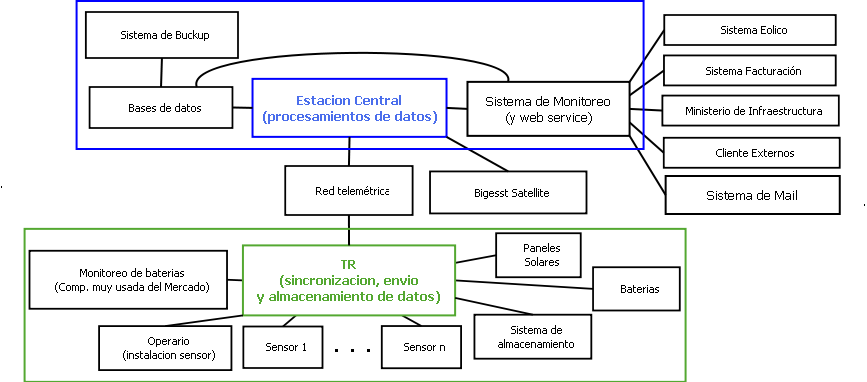
\includegraphics
[scale=0.5]{DiagramaConceptual.png}
\caption{\small Diagrama conceptual del sistema.}
\end{figure}

Como se puede observar, el sector de la Estaci�n Central, esta compuesta de una parte central, que es la encargada de procesar todos los datos que se reciban de las TRs, verificarlos, y seg�n el caso, identificar aquellos que no sean correctos, o correspondan a un outlier. Como indica la descripci�n del proyecto, la parte central es la encargada de comunicarse con el sistema Biggest Satelite, cuando se considere necesario obtener informaci�n de una zona cuando una TRs se cae y no es posible triangularla con  sus TRs vecinas, por este motivo, la estaci�n central esta relacionada directamente con Biggest Satelite. Adem�s de esta tarea, se realizan los c�lculos utilizando los modelos matem�ticos y los datos almacenados para realizar las predicciones sobre los desastres meteorol�gicos.

El modulo de Bases de Datos, corresponde al sector encargado de guardar todos los datos que las TRs env�en (previamente, procesados por la parte central) y otros como los resultados de los modelos matem�ticos que se computen. Es Sistema de Backup complementa al de Bases de Datos, teniendo la informaci�n redundante, y de esta forma impedir perdida de datos.

En el Sistema de Monitoreo, se encuentran las interfaces con todos los clientes y usuarios que utilicen el sistema, es decir, que en este modulo se implementaran las funcionalidades que corresponden con la comunicaci�n de sistemas externos que est�n interesados obtener informaci�n del sistema central, adem�s de los usuarios que tienen acceso al estado en tiempo real del sistema y puedan realizar cambios, modificando el comportamiento del sistema (por ejemplo, cambiando la agenda de un sensor).

Con respecto al sector que agrupa los m�dulos de la Terminal Remota, se encuentra la parte central, encargada de recibir, almacenar y enviar los datos que cada uno de los sensores brinda. Como el protocolo de envio tiene que ser confiable, cada dato enviado es guardado en el Sistema de Almacenamiento hasta que se confirme su llegada, de esta forma se esta contemplando uno de los requerimientos de proyecto, que es el de no tener perdida de datos.

Otra parte importante dentro del sector de la Terminal Remota, es el monitoreo de bater�as, que esta representado f�sicamente por un componente muy usado en el mercado. Este es el encargado de indicarle a la parte central de la TR cuando debe cambiar y utilizar la energ�a solar, por medio de los paneles solares, y cuando utilizar la energ�a almacenada dentro de las bater�as.



\clearpage

\newpage
\chapter{Planificaci�n del Proyecto}

\section{Generaci�n y descripci'on de Casos de Uso}

En el siguiente texto se mostrar'an los casos de uso principales identificados en el sistema, junto con su descripci'on. En algunos casos, se incluir'an tambien los diferentes actores, que participan en el mismo, 'estos se corresponden con los actores que se muestran en el diagrama de contexto del sistema.

\subsubsection{Indice de casos de Uso}

\subsubsection{Terminal Remota - TR}

\begin{itemize}
	\item TR01. Configurando agenda en sensor
	\item TR02. Obteniendo datos censados
	\item TR03. Monitoreando/configurando consumo de energ�a 
	\item TR04. Detectando ca�da del sensor
	\item TR05. Detectando recuperaci�n del sensor 
	\item TR06. ABM de sensor
	\item TR07. Detectando posible ca�da por falta de energ�a
	\item TR08. Recuperando luego de ca�da por falta de energ�a
	\item TR09. Sincronizando datos de censados
	\item TR10. Encriptando, comprimiendo y enviando mensaje seg�n protocolo
	\item TR11. Repitiendo mensaje al no tener confirmaci�n
	\item TR12. Borrando mensaje al llegar confirmaci�n
\end{itemize}

\subsubsection{Estaci�n Central - EC}

\begin{itemize}
	\item EC01. Marcando punto de restauraci�n de datos correctos del sistema
	\item EC02. Procesando modelos matem�ticos
	\item EC03. Notificando resultado del modelo
	\item EC04. Guardando datos del modelo
	\item EC05. Detectando caida/alta de TR
	\item EC06. Triangulando o reemplazando por BS TR/sensor
	\item EC07. Anunciando remplazo o triangulacion de TR/sensor
	\item EC08.	Normalizando TR/sensor y anunciandolo
	\item EC09. Detectando red congestionada y anunciandolo
	\item EC10. Detectando outliers y anunciandolo
	\item EC11.	Descartando � incluyendo posibles outliers
	\item EC12.	Ordenando y descartando mensajes repetidos
	\item EC13.	Confirmando llegada de mensaje
	\item EC14.	Guardando informaci�n de uso de Biggest Satelite
	\item EC15.	Definiendo intervalos de confianza para outliers
	\item EC16.	Obteniendo informaci�n e�lica del sistema del SM
	\item EC17.	Actualizando pautas en los modelos matem�ticos
	\item EC18.	Recibiendo, descomprimiendo y desencriptando mensaje de TR
	\item EC19. Recibiendo informaci�n de Biggest Satelite
	\item EC20.	Actualizando modelos para clientes externos
\end{itemize}

\subsubsection{Sistema de monitoreo - SM}

\begin{itemize}
	\item SM01.	Pidiendo datos del uso del servicio de Biggest Satelite
	\item SM02. Notificando ca�da de TR
	\item SM03.	Notificando red saturada 
	\item SM04.	Enviando datos al Min. de Infraestructura 
	\item SM05.	Enviando datos a cliente externo 
	\item SM06.	Recibiendo informaci�n del sistema e�lico
	\item SM07.	Configurando agenda dentro del sensor de una TR 
	\item SM08.	Configurando env�o de alertas
	\item SM09.	ABM de cliente externo
	\item SM10.	ABM de TR 
	\item SM11.	ABM de sensor 
	\item SM12.	Actualizando pantallas del monitoreo en tiempo real
\end{itemize}

\subsection{Casos de uso dentro de las TRs:}

\begin{enumerate}
\item Configurando agenda en sensor:
	\begin{itemize}
	\item Agentes: Estaci'on Central, Sensor.
	\item Descripci'on: La estaci�n central indica que se tiene que modificar la agenda de uno de los sensores de la TR, esta recibe las instrucciones, y modifica dicha agenda utilizando el protocolo de conexi�n con el sensor.
	\end{itemize}
	
\item Obteniendo datos censados:
	\begin{itemize}
	\item Agentes: Sensor.
	\item Descripci'on: La TR recibe un dato de un sensor y lo almacena para luego cuando llegue el tiempo correcto lo envie a la estacion central.
	\end{itemize}
	
\item Monitoreando/configurando consumo de energ�a:
	\begin{itemize}
	\item Agentes: Componente muy usada del mercado, Bater�a, Panel solar)
	\item Descripci'on: {\bf COMPLETAR}
	\end{itemize}

\item Detectando ca�da del sensor:
	\begin{itemize}
	\item Agentes: Estaci'on Central, Sensor.
	\item Descripci'on: Se detecta la caida de un sensor cuando la TR no recibe datos del mismo dentro del tiempo que tiene configurado para recibirlos. {\bf COMPLETAR}
	\end{itemize}
	
\item Detectando recuperaci�n del sensor:
	\begin{itemize}
	\item Agentes: Estaci'on Central, Sensor.
	\item Descripci'on:	Se detecta la reactivaci�n de un sensor cuando se comienza a recibir informaci�n del mismo. {\bf COMPLETAR}
	\end{itemize}
	
\item ABM de sensor:
	\begin{itemize}
	\item Agentes: Sensor, Operario, {\bf Estaci'on Central?}
	\item Descripci'on: Se instala un nuevo sensor en la TR y el operario la configura para que en determinado momento se comience a enviar sus datos a la Estaci�n Central.
	\end{itemize}

\item Detecci�n de posible ca�da por falta de energ�a:
	\begin{itemize}
	\item Agentes: Componente muy usada del mercado, Estaci'on Central.
	\item Descripci'on: El componente muy usado del mercado le indica a la TR que la energ�a en la bater�a se encuentra en un nivel bajo y es necesario recargarla, en este caso ls TR indica esto a la estaci�n central. {\bf COMPLETAR}
	\end{itemize}

\item assdfasdf
	\begin{itemize}
	\item Agentes:
	\item Descripci'on:
	\end{itemize}
	
\end{enumerate}


\section{Estimaciones a los casos de uso del proyecto(Asignaci�n de pesos)}

El m�todo que se utiliz� para estimar las tareas fue Wideban Delphi. A continuaci�n se detallar�n las principales etapas del proceso, sus complicaciones, resultados en com�n y las conclusiones finales.

\subsection{Planificaci�n y reuni�n de lanzamiento}

Estas dos etapas del proceso fueron b�sicamente, para poner en com�n que se iban a estimar los casos de uso de la secci�n anterior, el m�todo utilizado, y la medida que se iba a utilizar para la estimaci�n, en nuestro caso llegamos a que la medida para estimar viene dada por d�as/persona teniendo en cuenta d�as de 24 horas. Esta decicion fue tomada m�s que nada para simplificar la estimaci�n y no tener que trabajar en horas en esta parte del proyecto. El objetivo b�sico de �stas estimaciones fue para poder luego determinar cantidad de iteraciones, duraci�n y fase a la que pertenecen de manera m�s o menos objetiva. Los encargados de llevar a cabo las estimaciones fuimos los 4 integrantes del grupo.

\subsection{Preparaci�n individual y reuni�n de estimaci�n}

En estas dos etapas del proceso llevamos a cabo cada uno las estimaciones que consideramos necesarias para cada uno de los casos de uso. Luego analizamos diferencias realizando gr�ficos que reflejaran la informaci�n de las estimaciones como se detalla a continuaci�n.

La primera ronda de estimaciones genero los siguientes resultados:

\begin{figure}[H]
  \centering
    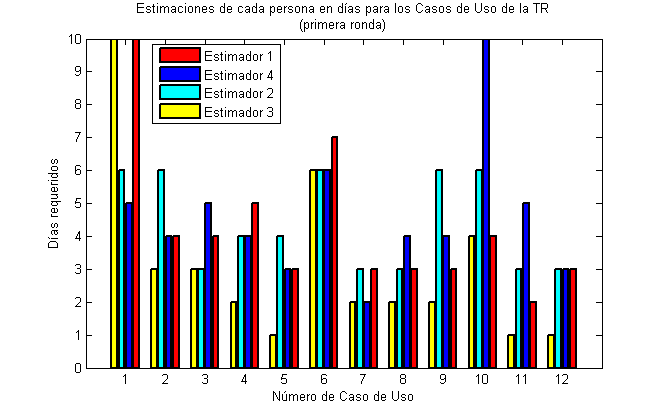
\includegraphics[width=13cm,height=6cm]{EstimacionTR1raRonda.png}
\end{figure}

\begin{figure}[H]
  \centering
    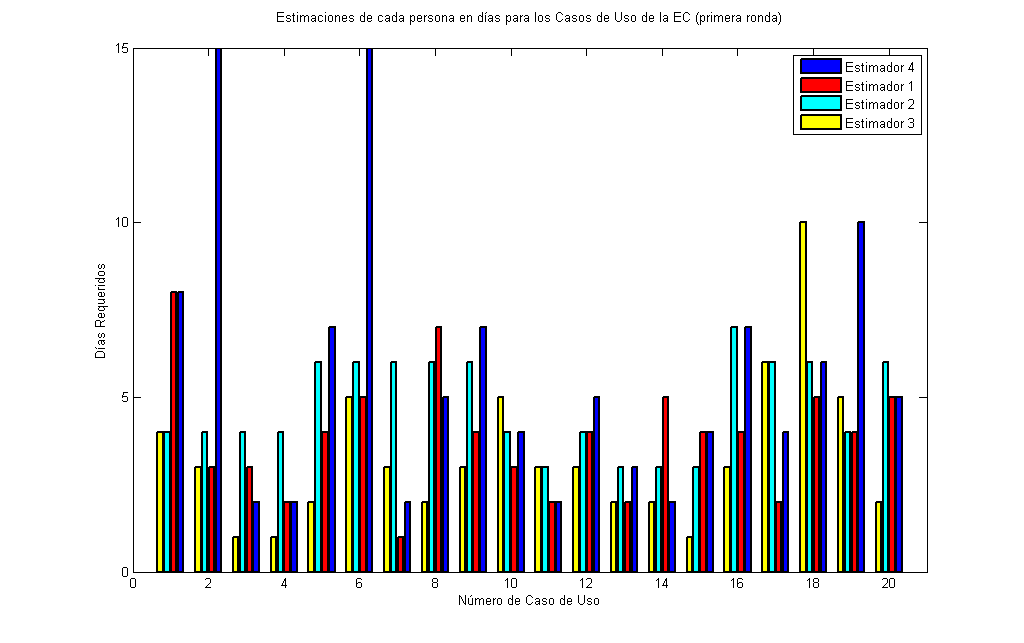
\includegraphics[width=13cm,height=6cm]{EstimacionEC1raRonda.png}
\end{figure}

\begin{figure}[H]
  \centering
    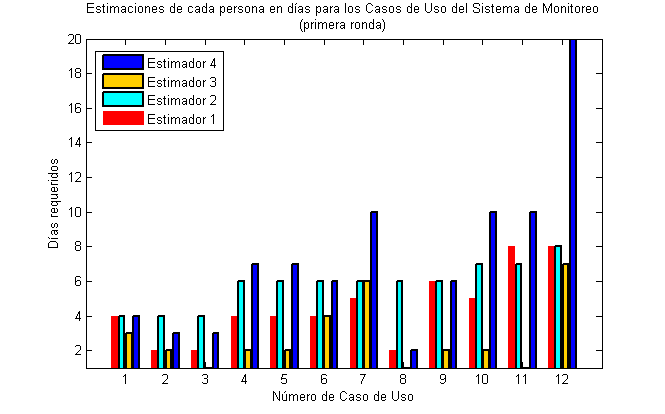
\includegraphics[width=13cm,height=6cm]{EstimacionSM1raRonda.png}
\end{figure}

\clearpage
\newpage

Hab�a muchas tareas que difer�an bastante en la estimaci�n por lo cual en la primera reuni�n de estimaci�n se intent� nuevamente ver el alcance de cada caso de uso, lo cual sirvi� para que algunos estimadores pudieran tener en cuenta tareas y funcionalidades que en principio no habian considerado. Luego se procedi� a realizar una segunda ronda de estimaciones y los resultados se detallan a continuaci�n en los siguientes gr�ficos:

\begin{figure}[H]
    \centering
    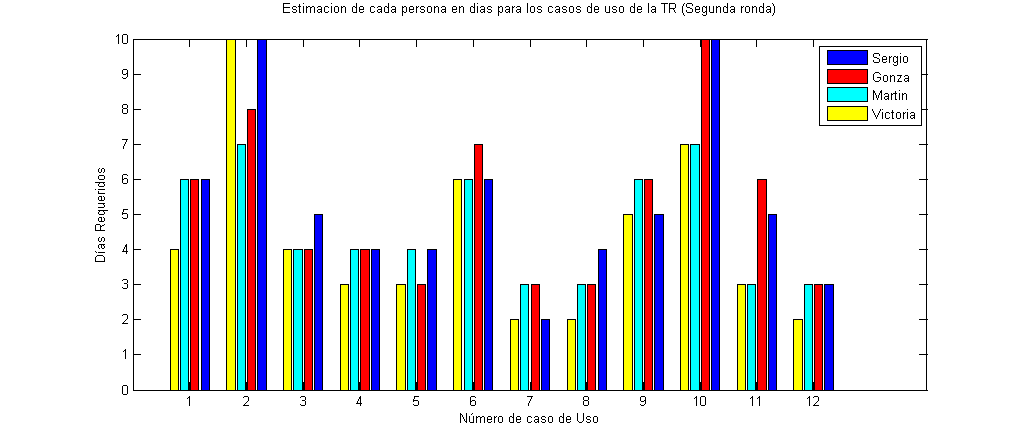
\includegraphics[width=13cm,height=6cm]{EstimacionTR2daRonda.png}
\end{figure}

\begin{figure}[H]
    \centering
    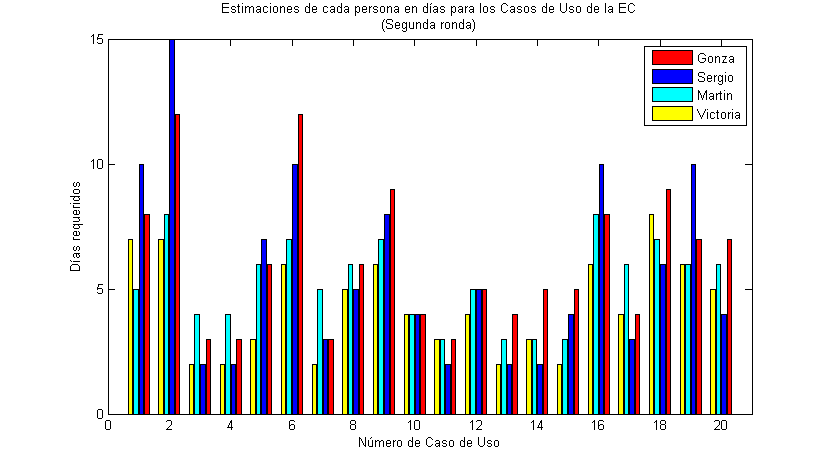
\includegraphics[width=13cm,height=6cm]{EstimacionEC2daRonda.png}
\end{figure}

\begin{figure}[H]
    \centering
    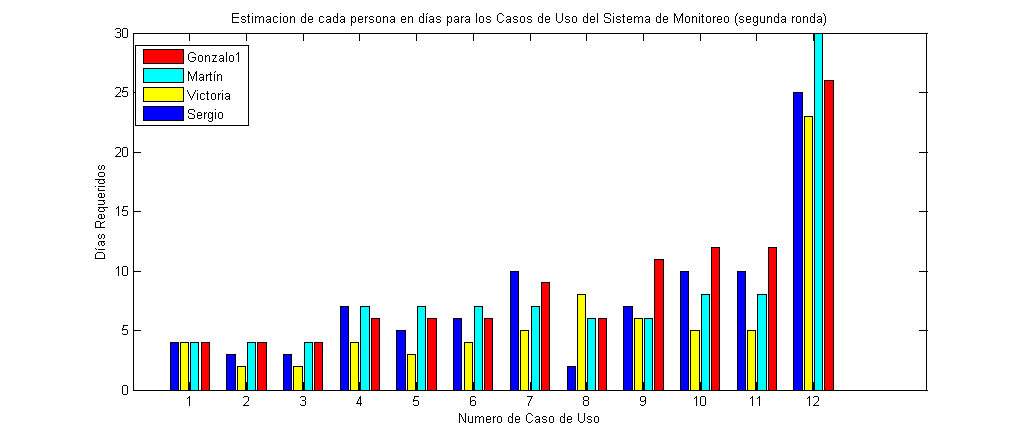
\includegraphics[width=13cm,height=6cm]{EstimacionSM2daRonda.png}
\end{figure}


\clearpage
\newpage

Si bien hubo mejor�as en la segunda ronda, consideramos que exist�an desv�os no aceptables, por lo cual nuevamente se revisaron los casos de uso y se lleg� a la concluci�n que una tercera ronda de estimaciones reducir�a �stos desv�os. Luego de la tercera ronda consideramos detener las estimaciones ya que el desv�o fue aceptable (alrededor de dos d�as )y las estimaciones, calculando un promedio entre ellas pod�an llegar a reflejar valores adecuados. Los resultados son los siguientes: 

\begin{figure}[H]
    \centering
    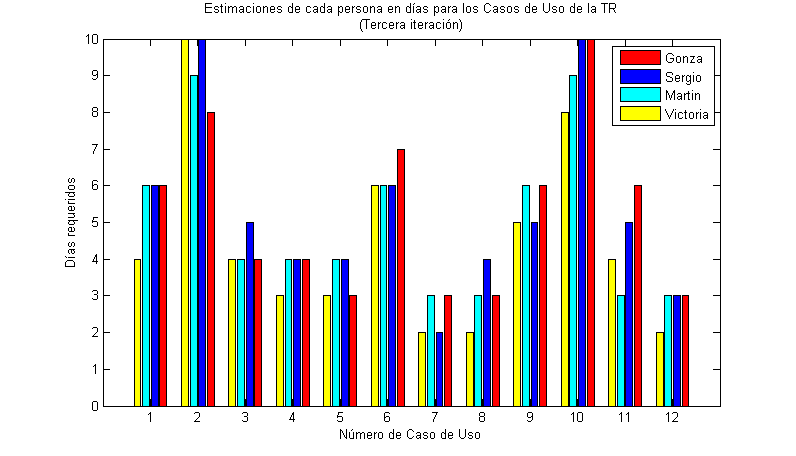
\includegraphics[width=13cm,height=6cm]{EstimacionTR3raRonda.png}
\end{figure}

\begin{figure}[H]
    \centering
    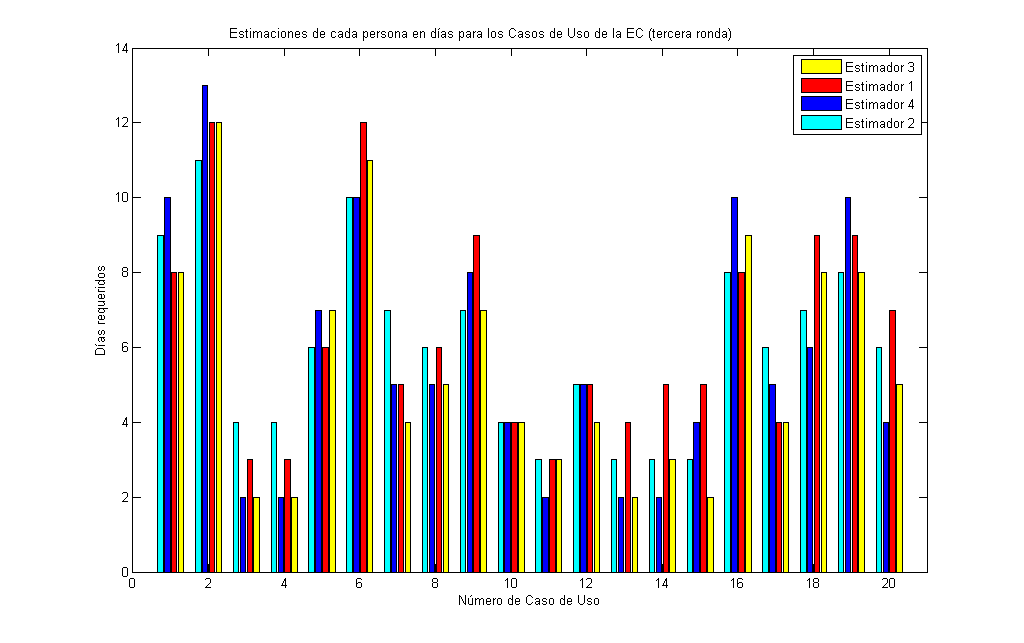
\includegraphics[width=13cm,height=6cm]{EstimacionEC3raRonda.png}
\end{figure}

\begin{figure}[H]
    \centering
    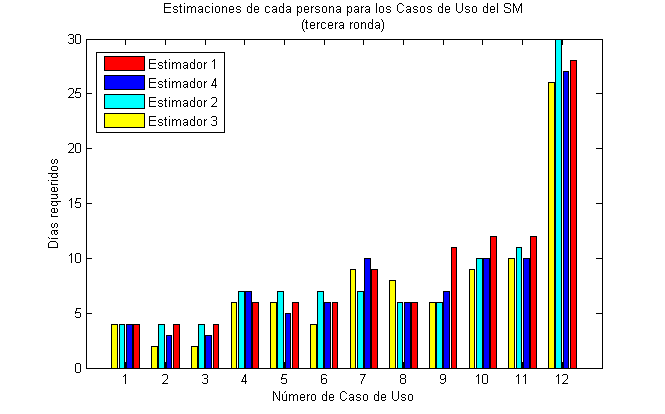
\includegraphics[width=13cm,height=6cm]{EstimacionSM3raRonda.png}
\end{figure}


\clearpage
\newpage
\subsection{Ensamblado de tareas y revisi�n de resultados}

Finalemnte en �sta secci�n se calcul� un promedio de las estimaciones realizadas para cada tarea por cada estimador y se pudo conclu�r en resultados que a todos los integrantes le parecieron adecuados. A continuaci�n se detallan los pesos asigandos a cada caso de uso que resultaron del proceso de estimaci�n.

\begin{itemize}

\item Casos de uso de la TR.
	
\begin{tabular}{||l | r||}
\hline
\hline
N�mero CU & Duraci�n \\
\hline
 CU 1  & 5 \\
\hline
 CU 2  & 9 \\
\hline 
 CU 3  & 4 \\
\hline
 CU 4  & 3 \\
\hline
 CU 5  & 3 \\
\hline
 CU 6  & 6 \\
\hline
 CU 7  & 2 \\
\hline
 CU 8  & 3 \\
\hline
 CU 9  & 5 \\
\hline
 CU 10  & 9 \\
\hline
 CU 11  & 4 \\
\hline
 CU 12  & 2 \\
\hline
\hline
\end{tabular}
\newline

\item Casos de uso de la EC.
	
\begin{tabular}{||l | r||}
\hline
\hline
N�mero CU & Duraci�n \\
\hline
 CU 1  & 8 \\
\hline
 CU 2  & 12 \\
\hline 
 CU 3  & 2 \\
\hline
 CU 4  & 2 \\
\hline
 CU 5  & 6 \\
\hline
 CU 6  & 10 \\
\hline
 CU 7  & 5 \\
\hline
 CU 8  & 5 \\
\hline
 CU 9  & 7 \\
\hline
 CU 10  & 4 \\
\hline
 CU 11  & 2 \\
\hline
 CU 12  & 4 \\
\hline
 CU 13  & 2 \\
\hline
 CU 14  & 3 \\
\hline
 CU 15  & 3 \\
\hline
 CU 16  & 8 \\
\hline
 CU 17  & 4 \\
\hline
 CU 18  & 7 \\
\hline
 CU 19  & 8 \\
\hline
 CU 20  & 5 \\
\hline
\hline
\end{tabular}
\newline

\item Casos de uso del SM.
	
\begin{tabular}{||l | r||}
\hline
\hline
N�mero CU & Duraci�n \\
\hline
 CU 1  & 4 \\
\hline
 CU 2  & 3 \\
\hline 
 CU 3  & 3 \\
\hline
 CU 4  & 6 \\
\hline
 CU 5  & 6 \\
\hline
 CU 6  & 5 \\
\hline
 CU 7  & 8 \\
\hline
 CU 8  & 6 \\
\hline
 CU 9  & 7 \\
\hline
 CU 10  & 10 \\
\hline
 CU 11  & 10\\
\hline
 CU 12  & 27 \\
\hline
\hline
\end{tabular}

\end{itemize}
\clearpage

\newpage
\chapter{Planificaci�n de la primera iteraci�n}
\clearpage

\newpage
\chapter{Conclusi�n}

Si bien se sabe que el dise�o del proyecto est� en sus primeros pasos, con lo realizado en esta preentrega, se tiene una especificaci�n relativamente exhaustiva de las cosas mas importantes del dominio del problema. Con estos datos se pudo definir la base de la arquitectura del sistema, que si bien puede cambiar, se supone que no afectara gravemente el dise�o original, ni traer� problemas que posterguen demasiado el proyecto.

Para realizar esta afirmaci�n nos basamos en que al realizar el diagrama contextual (que sirve en este caso de arquitectura), tomamos en cuenta varios de los requerimientos y atributos de calidad planteados inicialmente, proponiendo una arquitectura que es incremental, en cuanto a que se pueden agregar Terminales Remotas, y en cuanto a que se puede incrementar el poder de c�mputo. Tambi�n es resistente a fallas en las transmisiones, ya que se implementara un protocolo confiable entre las TRs y la Estaci�n Central y tambi�n es resistente a fallas en los equipos, dado que se van a poder subsanar la ca�da de una TR triangulando o utilizando un servicio externo. Adem�s se contempla el hecho de tener comunicaci�n con diferente tipo de sistemas, ya sean clientes externos (como AgroTop), proveedores de servicio (Biggest Satelite) y usuarios internos, encargados de monitorear el estado del sistema.

Se dise�� un plan que tiene en cuenta tiempos de entrega y de desarrollo que son acotados, por esta raz�n se tuvo que identificar dependencias entre las funcionalidades principales que se detectaron, como as� su importancia y complejidad dentro del sistema.

Como se conoce estos m�todos llevan bastante tiempo, pero ayudan a tener un control del proyecto y tener luego un hilo de ejecuci�n bien definido que permitir� optimizar el desarrollo del sistema durante el tiempo. Teniendo en cuenta el contexto en el que se realiz� el trabajo creemos haber cumplido las expectativas en cuanto a los requerimientos pedidos para esta entrega.

\clearpage
\label{LastPage}
\end{document}
